%!TEX root = main.tex
\section{Details in Section~\ref{sec:symbolic}}\label{app-sym}

\subsection{The construction of an equivalent \SA{} from a \SSA{}(the first claim of Proposition~\ref{prop-2nsa})}

Let $\Aut = (\Upsilon, \EndLeft, \EndRight, \controls, q_0, \finals, \transrel)$ be a \SSA. We show how to construct an equivalent \SA{} $\Aut' =  (\Upsilon, \controls', q'_0, \finals', \transrel')$.
W.l.o.g., we assume that for each transition $(q, \psi, dir, q') \in \transrel$, we have $dir \in \{\Left,\Right\}$. Every \SSA{} can be turned into one \SSA{} satisfying the assumption as follows: Replace each transition $(q, \psi, \Stay, q') \in \transrel$ with three new transitions $(q, \psi, \Right, q'')$, $(q'', \ltrue, \Left, q')$, and $(q'', \EndRight, \Left, q')$, where $q''$ is a fresh state.

The proof is an adaptation of the construction of \FA{} from \FFA{} based on the notion of crossing sequences (cf., e.g., \cite{HU79}). Since \SSA{}s replace the letters in \FFA{}s with unary predicates, the main technical challenge here is to deal with these predicates (i.e., guards).

We first use an example to illustrate the idea of crossing sequences: Suppose $w = \EndLeft d_1 d_2 d_3 d_4 d_5\EndRight$, and an accepting run of $\Aut$ on $w$ uses the following sequence of transitions 
\[
\begin{array}{l}
(q_0, \EndLeft, \Right, q_1), (q_1, \psi_1, \Right, q_1), (q_1, \psi_2, \Left, q_2), (q_2, \psi_3, \Right, q_0), (q_0, \psi_4, \Right, q_1), \\
(q_1, \psi_1, \Right, q_1), (q_1, \psi_1, \Right, q_1), (q_1, \psi_2, \Left, q_2), (q_2, \psi_3, \Right, q_0), (q_0, \psi_4, \Right, q_1),
\end{array}
\] 
with $q_1 \in \finals$.
(The run is illustrated in Figure~\ref{fig-2sa-sa}.) A \emph{crossing sequence} of the run is a sequence of states on the boundary of two tape cells, e.g. the sequence $q_1, q_2, q_0$ on the boundary of $d_1$ and $d_2$. Note that for technical convenience, the states of the run are put in a way that, whenever a left-transition $(q, \psi, \Left, q')$ is taken, $q'$ is put just below $q$, thus in the \emph{same} crossing sequence as $q$ rather than the cross sequence of th position on the left. Therefore, 
\emph{the target state of each left-transition is put in the position right-adjacent to the actual position of the reading head}.
For instance, in Figure~\ref{fig-2sa-sa}, when the transition $(q_1, \psi_2, \Left, q_2)$ is taken, $q_2$ is put just below $q_1$. Different from the crossing sequences for 2FAs, in Figure~\ref{fig-2sa-sa}, naturally we also include the guards of the transitions. 

\begin{figure}[htbp]
\begin{center}
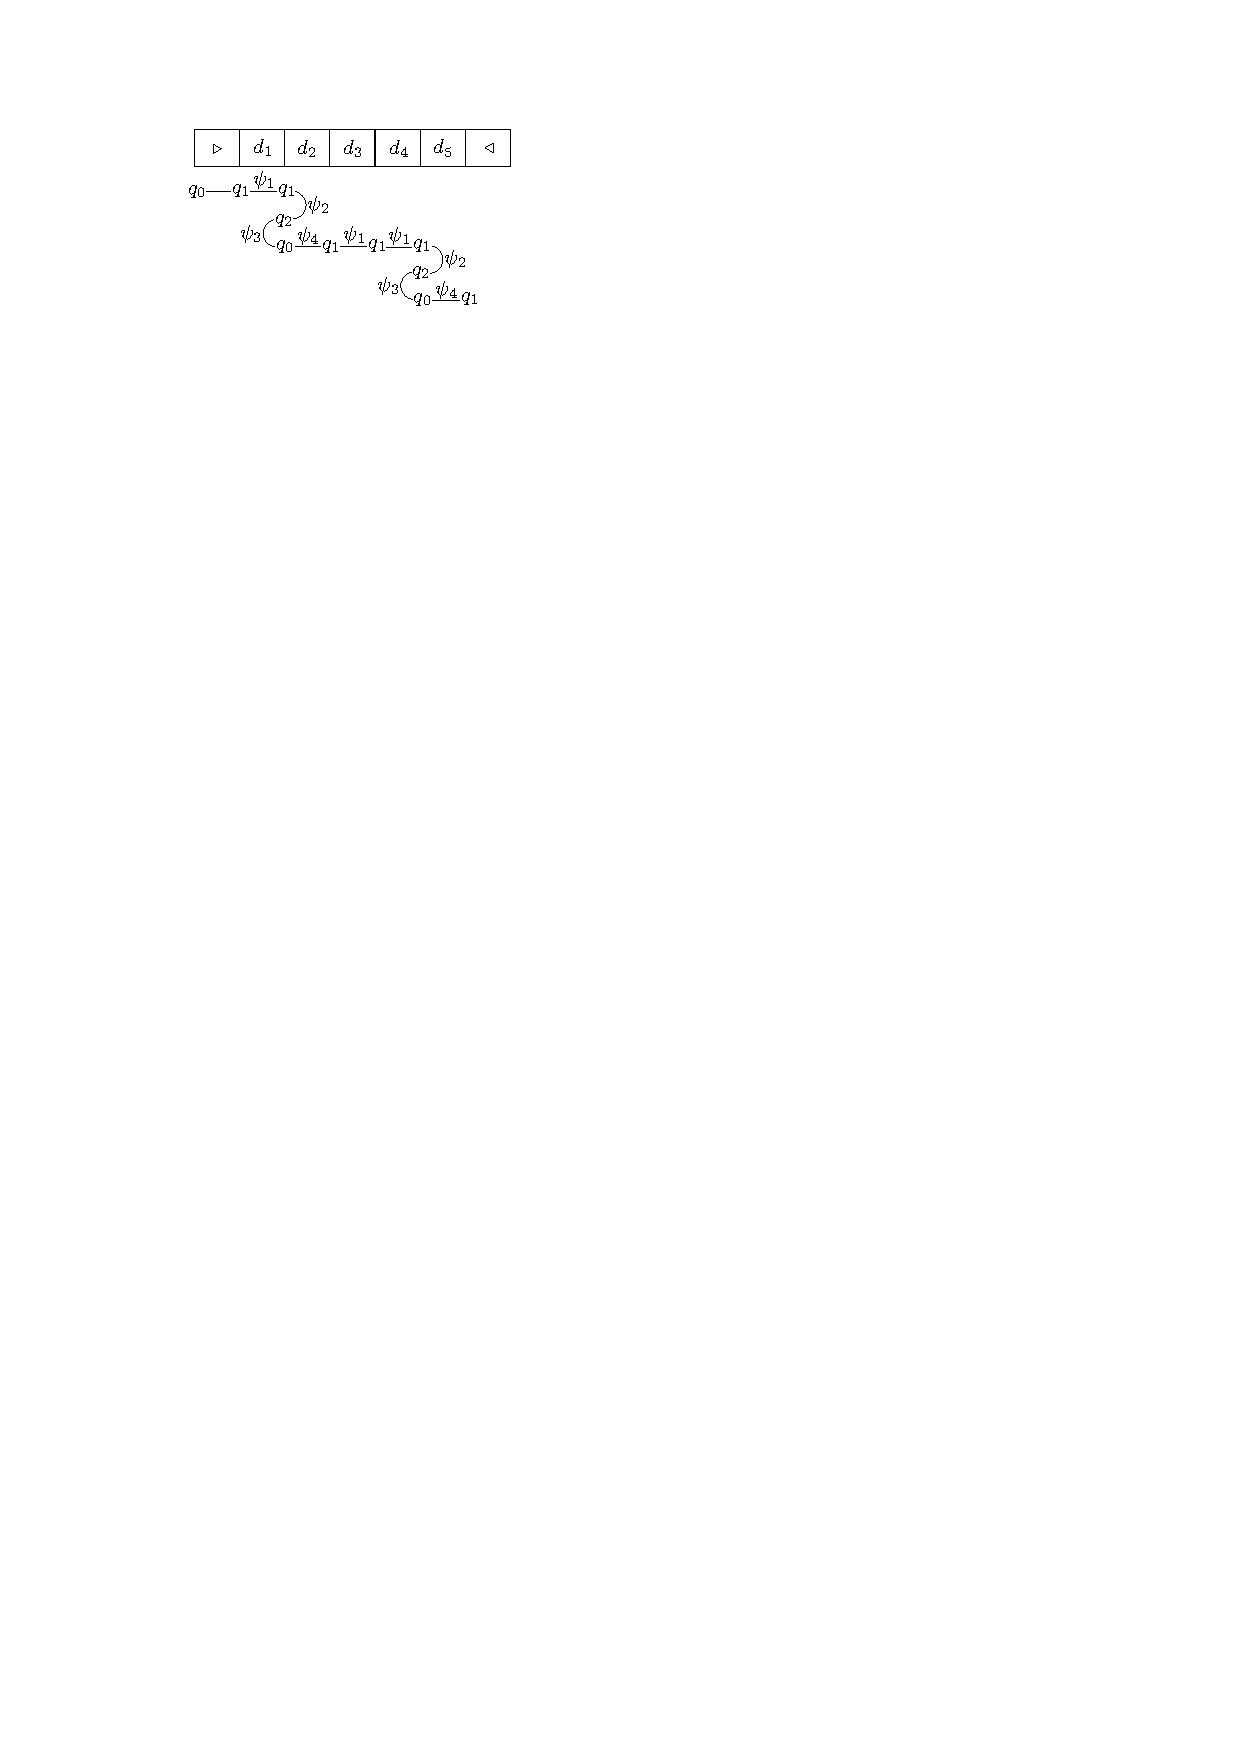
\includegraphics{2sa-sa-exmp.pdf}
\end{center}
\caption{Accepting runs of $\Aut$: An example}\label{fig-2sa-sa}
\end{figure}

In order to deal with the guards in the transitions, we adapt the crossing sequences of the \SSA{} $\Aut$  as follows: a crossing sequence of $\Aut$ is a sequence of \emph{transitions} of odd lengths such that  the source states of the transitions in the even and odd  positions respectively are mutually distinct. Let $S_\transrel$ denote the set of such sequences of transitions. 
%Notice that, in general, any $\rho\in S_\transrel$  is of the form that $\rho = \tau_1, \ldots, \tau_{2n+1}$ for some $n$ such that for each $i \in [n+1]$, $\tau_{2i-1} = (p_{2i-1}, \EndRight, \Left, q_{2i-1})$, and for each $i \in [n]$, $\tau_{2i} = (p_{2i}, \psi_{2i}, dir_{2i}, q_{2i})$.


\newcommand\lmatch{\mathsf{LeftMatch}}
\newcommand\rmatch{\mathsf{RightMatch}}

In order to construct the set of transitions of $\Aut'$, we shall define two \emph{partial} functions $\lmatch(\rho_1, \rho_2)$ and $\rmatch(\rho_1, \rho_2)$ for $\rho_1, \rho_2 \in S_\transrel$. 
The intention of $\lmatch(\rho_1, \rho_2)$ and $\lmatch(\rho_1, \rho_2)$ is explained as follows.
\begin{itemize}
\item The intention of $\lmatch(\rho_1, \rho_2)$: $\rho_1$ and $\rho_2$ are the crossing sequences to the left resp. right of some position $i$ holding a data value $d$. Initially, we reach the source state of the first transition of $\rho_2$ by a \emph{left-transition} (thus after this transition, the reading head is in the position $i$\footnote{Recall that the target state of each left-transition is put in the position right-adjacent to the actual position of the reading head.}).
%
\item The intention of $\rmatch(\rho_1, \rho_2)$:  $\rho_1$ and $\rho_2$ are the crossing sequences to the left resp. right of some position $i$ holding a data value $d$. Initially, we reach the source state of the first transition of $\rho_1$ %, say $p_1$, 
by a \emph{right-transition} (thus after this transition, the reading head is in the position $i$).
\end{itemize}
%
Formally, the domain of $\lmatch$ (resp. $\rmatch$) is defined inductively as follows, where in each case below, the return value is also specified. Let $\rho_1, \rho_2 \in S_\transrel$. Then $\lmatch(\rho_1, \rho_2)$ is defined iff one of the following constraints holds.
\begin{itemize}
\item Case $\rho_1 = \varepsilon$, $\rho_2 = \varepsilon$: $\lmatch(\rho_1, \rho_2) = \ltrue$.
%
\item Case $\rho_1 =  \tau_{1,1}, \ldots, \tau_{1,k}$ with $k \ge 1$, $\rho_2 = \tau_{2,1}, \ldots, \tau_{2,l}$ with $l \ge 1$, $\tau_{2,1} = (q_1, \psi_{2,1}, \Left, p_1)$, $p_1$ is the source state of $\tau_{1,1}$, and $\rmatch(\rho'_1, \rho'_2)$ is defined:  
$$\lmatch(\rho_1, \rho_2) = \psi_{2,1} \wedge \rmatch(\rho'_1, \rho'_2),$$ 
where $\rho'_1 = \tau_{1,2}, \ldots, \tau_{1,k}$ and $\rho'_2 = \tau_{2,2}, \ldots, \tau_{2,l}$.
%
\item Case $\rho_1 =  \tau_{1,1}, \ldots, \tau_{1,k}$ with $k \ge 1$, $\rho_2 = \tau_{2,1}, \ldots, \tau_{2,l}$ with $l \ge 1$, $\tau_{2,1} = (q_1, \psi_{2,1}, \Right, q_2)$, $q_2$ is the source state of $\tau_{2,2}$, and $\lmatch(\rho_1, \rho'_2)$ is defined:  
$$\lmatch(\rho_1, \rho_2) = \psi_{2,1} \wedge \lmatch(\rho_1, \rho'_2),$$ 
where $\rho'_2 = \tau_{2,3}, \ldots, \tau_{2,l}$.
%
\end{itemize} 
%
Symmetrically, $\rmatch(\rho_1, \rho_2)$ is defined iff one of the following constraints holds.
\begin{itemize}
\item Case $\rho_1 = \varepsilon$, $\rho_2 = \varepsilon$: $\rmatch(\rho_1, \rho_2) = \ltrue$.

\item Case $\rho_1 =  \tau_{1,1}, \ldots, \tau_{1,k}$ with $k \ge 1$, $\rho_2 = \tau_{2,1}, \ldots, \tau_{2,l}$ with $l \ge 1$, $\tau_{1,1} = (p_1, \psi_{1,1}, \Right, q_1)$, $q_1$ is the source state of $\tau_{2,1}$, and $\lmatch(\rho'_{1}, \rho'_2)$ is defined:  
$$\rmatch(\rho_1, \rho_2) =\psi_{1,1} \wedge \lmatch(\rho'_{1}, \rho'_2),$$ 
where $\rho'_1 = \tau_{1, 2},\ldots, \tau_{1,k}$, and $\rho'_2 = \tau_{2,2}, \ldots, \tau_{2,l}$.
%
\item Case $\rho_1 =  \tau_{1,1}, \ldots, \tau_{1,k}$ with $k \ge 1$, $\rho_2 = \tau_{2,1}, \ldots, \tau_{2,l}$ with $l \ge 1$, $\tau_{1,1} = (p_1, \psi_{1,1}, \Left, p_2)$, $p_2$ is the source state of $\tau_{1,2}$, and $\rmatch(\rho'_1, \rho_2)$ is defined:  
$$\rmatch(\rho_1, \rho_2) = \psi_{1,1} \wedge \rmatch(\rho'_1, \rho_2),$$ 
where $\rho'_1 = \tau_{1,3}, \ldots, \tau_{1,k}$.
%
\end{itemize}
%
We are ready to construct the \SA{} $\Aut' =  (\Upsilon, \controls', q'_0, \finals', \transrel')$, where
\begin{itemize}
\item $\controls' = S_\transrel \cup \{q'_0\}$, where $q'_0$ is a fresh state,
%
\item $\finals'$ comprises the set of elements $\rho \in S_\transrel$ as follows: suppose $\rho = \tau_1, \ldots, \tau_{2n+1}$, where for each $i \in [n+1]$, $\tau_{2i-1} = (p_{2i-1}, \EndRight, \Left, q_{2i-1})$, and for each $i \in [n]$, $\tau_{2i} = (p_{2i}, \psi_{2i}, dir_{2i}, q_{2i})$, then $\rho$ must satisfy that $q_{2n+1} \in F$ and $q_{2i-1} = p_{2i}$ for each $i \in [n]$,  
%
\item $\transrel'$ comprises the following transitions: 
%
\begin{itemize}
%
\item $(\rho, \rmatch(\rho, \rho'), \rho') \in \transrel'$ for all $\rho, \rho' \in S_\transrel$ such that $\rmatch(\rho, \rho')$ is defined;
%
\item  
%the transitions out of $q'_0$ are defined as follows:
%
$(q'_0, \rmatch(\rho, \rho'), \rho') \in \transrel'$ for all $\rho \in I'$ and $\rho' \in S_\transrel$ such that $\rmatch(\rho, \rho')$ is defined, where 
$I'$ comprises $\rho'' \in S_\transrel$ satisfying the following constraints: $\rho'' = \tau_1, \ldots, \tau_{2n+1}$,  for each $i \in [n+1]$, $\tau_{2i-1} = (p_{2i-1}, \psi_{2i-1}, dir_{2i-1}, q_{2i-1})$, for each $i \in [n]$, $\tau_{2i} = (p_{2i}, \EndLeft, \Right, q_{2i})$. In addition, $(q_0, \EndLeft, \Right, p_1) \in \transrel$, and for each $i \in [n]$, $q_{2i} = p_{2i+1}$. 
\end{itemize}
%
\end{itemize}

Since $S_\transrel$ contains at most $(|\Aut|_c)^{2 |\controls|-1} \le (|\Aut|_c)^{2 |\Aut|_c}$ elements, we conclude that 
$$
\begin{array}{l c l}
|\Aut'|_c \le ((|\Aut|_c)^{2|\Aut|_c})^2  & = & (|\Aut|_c)^{4|\Aut|_c} 
 \approx    2^{\bigO\left(|\Aut|_c \log |\Aut|_c\right)}
\end{array}
$$ 
and 
$$
\begin{array}{l c l}
|\Aut'|_d \le 2(2|\controls|-1) |\Aut|_d & \le & 4 |\Aut|_c |\Aut|_d 
\approx   \bigO( |\Aut|_c |\Aut|_d).
\end{array}
$$




%%%====================================================================
%%%====================================================================

\subsection{Complexity of the generic decision procedure (Theorem~\ref{thm-generic-dec-symbolic})}

For each $i$, let $M_i$ be the maximum number of elements in $\cE_i(x)$ for $x  \in \vars(S)$,
and $N_{i,s}$ (resp. $N_{i, d}$) be the maximum structural size (resp. data size) of the conjunctive \SA{}s in $\bigcup \limits_{x \in \vars(S)} \cE_i(x)$. Then we have $M_{i-1} \le (\rcdim(S)+1)M_i $. Moreover, since each string function $f$ satisfies  $|f|_s \le \rcphi_s(S)$, we have 
%
$$N_{i-1, s} \le \ell_s(|f|_s, N_{i, s}) \le \ell_s(\rcphi_s(S), N_{i,s})$$ 
%
Moreover, since $|f|_s \le \rcphi_s(S)$ and $|f|_d \le \rcphi_d(S)$, we have
%
$$N_{i-1, d} \le \ell_d(|f|_s, |f|_d, N_{i, c}, N_{i,d}) \le \ell_d(\rcphi_s(S), \rcphi_d(S), N_{i, s}, N_{i,d}).$$ 

Because for each $x \in \vars(S)$, $\cE_{\rcdep(S)}(x)$ contains at most $\rcsreg(S)$ elements, we have that for each $x \in \vars(S)$, $\cE(x)$ contains at most $(\rcdim(S)+1)^{\rcdep(S)}\rcsreg(S)$ elements. 
Moreover, because each conjunctive \SA{} in $\cE_{\rcdep(S)}(x)$ satisfies that its control and data size are bounded by $\rcpsi_c(S)$ and $\rcpsi_d(S)$ respectively, 
we have that each conjunctive \SA{} in $\cE(x)$ satisfies that its control and data size are bounded by $\ell_s^{\langle \rcdep(S) \rangle}(\rcphi_s(S), \rcpsi_s(S))$ and 
%
\[ (\ell_d)^{\langle  \rcdep(S) \rangle}_{\ell_s}(\rcphi_s(S), \rcphi_d(S), \rcpsi_s(S), \rcpsi_d(S)).\]
% h(i, j, g^{\langle n \rangle}(k, l), h^{\langle n \rangle}(i, j, k, l))
% 
We emphasise that, according to the $\mathbb{S}$\prerec{} assumption, the construction of these \SA{}s can be done in nondeterministic space bounded by
%
{
\small
$$\ell_c^{\langle  \rcdep(S) \rangle}(\rcphi_s(S), \rcpsi_s(S)) \cdot (\ell_d)^{\langle \rcdep(S) \rangle}_{\ell_c}(\rcphi_s(S),  \rcphi_d(S), \rcpsi_s(S), \rcpsi_d(S))$$
}
%
Therefore, for each $x \in \vars(S)$, the conjunctive product \SA{} $\Aut_x=((\controls_x, \transrel_x), S_x)$ of these conjunctive \SA{}s  in $\cE(x)$ has a structural size bounded by 
%
$$(\ell^{\langle \rcdep(S) \rangle}_s(\rcphi_s(S), \rcpsi_s(S)))^{(\rcdim(S)+1)^{\rcdep(S)} \rcsreg(S)},$$
%
and data size bounded by
%
\[ (\rcdim(S)+1)^{\rcdep(S)} \rcsreg(S) (\ell_d)^{\langle  \rcdep(S) \rangle}_{\ell_s}(\rcphi_s(S),\rcphi_d(S),  \rcpsi_s(S), \rcpsi_d(S)).\]
%
and $|S_x| \le (\ell_s^{\langle \rcdep(S) \rangle}(\rcphi_s(S), \rcpsi_s(S)))^2$. 
Therefore, the structural and data size of the (standard) \SA{} corresponding to $\Aut_x$ are  bounded by 
%
$$(\ell^{\langle \rcdep(S) \rangle}_s(\rcphi_s(S), \rcpsi_s(S)))^{(\rcdim(S)+1)^{\rcdep(S)} \rcsreg(S) (\ell_s^{\langle \rcdep(S) \rangle}(\rcphi_s(S), \rcpsi_s(S)))^2}$$
%
and
$$
\begin{array}{l}
(\ell_s^{\langle \rcdep(S) \rangle}(\rcphi_s(S), \rcpsi_s(S)))^2 (\rcdim(S)+1)^{\rcdep(S)} \rcsreg(S)\ \cdot  \\
\hspace{1cm}(\ell_d)^{\langle  \rcdep(S) \rangle}_{\ell_s}(\rcphi_s(S),\rcphi_d(S),  \rcpsi_s(S), \rcpsi_d(S))
\end{array}
$$
respectively.

Since the nonemptiness of an \SA{} $\Aut$ can be solved in nondeterministic $(\log |\Aut|_s) + \beta(|\Aut|_d)$ space, we conclude that the nonemptiness of $\Aut_x$ can be solved in nondeterministic space bounded by 
{\small
$$
\begin{array}{l}
(\rcdim(S)+1)^{\rcdep(S)} \cdot \rcsreg(S) \cdot (\ell_s^{\langle \rcdep(S) \rangle}(\rcphi_s(S), \rcpsi_s(S)))^2 \log (\ell^{\langle \rcdep(S) \rangle}_s(\rcphi_s(S), \rcpsi_s(S))) \\
\hfill +\beta
\left(
\begin{array}{l}
(\ell_s^{\langle \rcdep(S) \rangle}(\rcphi_s(S), \rcpsi_s(S)))^2 (\rcdim(S)+1)^{\rcdep(S)} \rcsreg(S)\ \cdot  \\
\hspace{1cm} (\ell_d)^{\langle  \rcdep(S) \rangle}_{\ell_s}(\rcphi_s(S),\rcphi_d(S),  \rcpsi_s(S), \rcpsi_d(S))
\end{array}
\right)
\end{array}
$$
}


In summary, the aforementioned nondeterministic algorithm takes  $M + \beta(M)$ space, where 
%
$$
\begin{array}{l c l}
M & = & |\vars(S)| \cdot (\rcdim(S)+1)^{\rcdep(S)}  \rcsreg(S) \cdot  (\ell_s^{\langle \rcdep(S) \rangle}(\rcphi_s(S), \rcpsi_s(S)))^{r}\ \cdot \\
& &  \hspace{1cm} (\ell_d)^{\langle  \rcdep(S) \rangle}_{\ell_s}(\rcphi_s(S),\rcphi_d(S),  \rcpsi_s(S), \rcpsi_d(S))
\end{array}
$$
%
for some constant $r > 0$.


%%%========================================
%F.3
%%%========================================

\subsection{Proof of Lemma~\ref{lem-spt}: $\mathbb{S}$\prerec{} assumption for \SSPT{}s and \SPT{}s}

We first consider \SSPT{}s. Assume a \SSPT{} $\Transducer=(Y, Q, q_0, F, \delta)$ with $Y = \{y_1,\cdots, y_k\}$ and a conjunctive \SA{} $\Aut = ((Q', \transrel'), S')$ with $S' \subseteq Q' \times Q'$. 

Similarly to \FFA{}s, for $q \in F$ and  $S_{y_1}, \cdots, S_{y_k} \subseteq Q' \times Q'$, we  introduce a conjunctive \SSA{} $\cB_{\Transducer, \Aut, S_{x_1}, \cdots, S_{x_k}, q} = ((\controls'', \transrel''), S'')$, where $Q'' = Q \times Q'$, $S'' = \{((q_0, p), (q, p')) \mid (p, p') \in S'\}$, and the transition relation $\transrel''$ comprises the tuples 
$((q_1, q'_1), \psi(x), dir, (q_2, q'_2))$ such that there are $\psi_0(x) \in \Psi$ and $\vec{t}$ satisfying that $(q_1, \psi_0(x), dir, q_2, \vec{t}) \in \transrel$, and one of the following constraints holds, 
\begin{itemize}
\item $\vec{t} = t_1(x) \ldots t_r(x)$ is a sequence of $\signature$-terms, there are transitions 
$$(p_{0}, \psi_1(x), p_{1}), \ldots, (p_{r-1}, \psi_r(x), p_r) \in \transrel'$$ 
such that $p_0 = q'_1$, $p_r = q'_2$, and $\psi = \psi_0 \wedge \psi_1[t_1(x)/x] \wedge \ldots \wedge \psi_r[t_r(x)/x]$,
%
\item $\vec{t} = \vec{t}_1 y_{i_1} \ldots \vec{t}_{r} y_{i_{r}} \vec{t}_{r+1}$ such that $r \ge 1$, $\vec{t}_j = t_{j, 1} \ldots t_{j, s_j}$ is a sequence of $\signature$-terms for each $j \in [r+1]$,  and $i_j \in [k]$ for each $j \in [r]$, let $N = (\sum \limits_{j \in [r]} (s_j+ 1)) +s_{r+1}$, then there are states $p_0, \ldots, p_{N} \in \controls'$ satisfying that $p_0 = q'_1$, $p_{N} = q'_2$,  
%
$$
\begin{array}{l}
p_0 \xrightarrow[\Aut]{\psi_{1,1}} p_1\ \ldots\ p_{|\vec{t}_1|-1} \xrightarrow[\Aut]{\psi_{1, s_1}} p_{|\vec{t}_1|} \xrightarrow{S_{y_{i_1}}} p_{|\vec{t}_1|+1}\ \ldots\\
p_{N - s_{r+1} - s_r -1} \xrightarrow[\Aut]{\psi_{r, 1}} p_{N - s_{r+1} - s_r } \ \ldots\ p_{N - |\vec{t}_{r+1}| - 2} \xrightarrow[\Aut]{\psi_{r, s_r}} p_{N-s_{r+1}-1}\\
 \xrightarrow{S_{y_{i_r}}} p_{N- s_{r+1}} \xrightarrow[\Aut]{\psi_{r+1, 1}} p_{N -s_{r+1}+1}\ \ldots\ p_{N - 1} \xrightarrow[\Aut]{\psi_{r+1,  s_{r+1}} } p_{N},
\end{array}
 $$ 
 and $\psi = \psi_0 \wedge \bigwedge \limits_{j \in [r+1], j' \in [s_j]} \psi_{j, j'} [\vec{t}_{j, j'}(x)/x].$
\end{itemize}
%
%
%\item Define $\cB_{\Transducer, \Aut, S_{x_1}, \cdots, S_{x_k}, q}$ as $((Q''', \delta'''), S')$, where $S' = \{(\vec{\rho}_1, \vec{\rho}_2) \mid  (q'_1,q'_2) \in S, \vec{\rho}_1[1] =(q_0,q'_1), \vec{\rho}_2[|\vec{\rho}_2|] = (q, q'_2) \}$.
%\end{enumerate} 
Evidently, $|S''| = |S'|$.  Let $L$ be the maximum length of sequences of $\signature$-terms in transitions of $\Transducer$. Then 
\begin{itemize}
\item the structural size of $\cB_{\Transducer, \Aut, S_{y_1}, \cdots, S_{y_k}, q}$ is at most $|\Transducer|_s |\Aut|_s^{L} \le |\Transducer|_s |\Aut|_s^{|\Transducer|_s}$,
\item  on the other hand, since the size of $\psi_1[t_1(x)/x] \wedge \ldots \wedge \psi_r[t_r(x)/x]$ is at most $|\Transducer|_d |\Aut|_d$, we deduce that the data size of $\cB_{\Transducer, \Aut, S_{y_1}, \cdots, S_{y_k}, q}$ is at most $|\Transducer|_d + L |\Transducer|_d |\Aut|_d \le |\Transducer|^2_d |\Aut|_d$.
\end{itemize}
%It is easy to see that  the control size of $\cB_{\Transducer, \Aut, S_{y_1}, \cdots, S_{y_k}, q}$ is at most $|\Transducer|_c |\Aut|_c $ and $|S''| = |S'|$.   

%For $S \subseteq Q' \times Q'$, let $\Aut[S]$ denote the product of $\Aut(q'_1, \{q'_2\})$ for $(q'_1,q'_2) \in S$ (cf. Section~\ref{sec:prelim}, {Operations of NFAs.}). Since $S$ contains at most $|Q'|^2=|\Aut|^2$ many elements, the size of $\Aut[S]$ is bounded by $|\Aut|^{|\Aut|^2} \approx 2^{O(|\Aut|^2 \log |\Aut|)}$.

Therefore, $\Pre_\Transducer(\Aut)$ is equal to 
\[
\bigcup_{S_{y_1}, \cdots, S_{y_k} \subseteq Q' \times Q', q\in F} \Lang(\cB_{\Transducer, \Aut, S_{y_1}, \cdots, S_{y_k},q}) \times \Lang(\Aut[S_{y_1}]) \times \cdots  \times \Lang(\Aut[S_{y_k}])\]

We conclude that $\Pre_\Transducer(\Aut)$ is a recognisable relation. 

In order to compute a representation of $\Pre_\Transducer(\Aut)$, we transform the conjunctive \SSA{} $\cB_{\Transducer, \Aut, S_{x_1}, \cdots, S_{x_k},q}$ to a union of conjunctive \SA{}s as follows: Transform $\cB_{\Transducer, \Aut, S_{y_1}, \cdots, S_{y_k}, q}$ into a one-way transition graph $(\controls''',\delta''')$. From Proposition~\ref{prop-2nsa}, $\controls'''$ are vectors of transitions of $\cB_{\Transducer, \Aut, S_{y_1}, \cdots, S_{y_k}, q}$ of lengths at most $2|\controls''|-1$. Then $\Lang(\cB_{\Transducer, \Aut, S_{x_1}, \cdots, S_{x_k},q})$ is the union of $\Lang(((\controls''',\delta'''), S''))$ for $S'' \subseteq \controls''' \times \controls''',$ which comprises nondeterministically selected pairs $(\vec{\rho}_1, \vec{\rho}_2) \in \controls''' \times \controls'''$, one for each $(p, p') \in S'$, such that $\vec{\rho}_1[1] = ((q_0, p), -, -)$ and  $\vec{\rho}_2[|\vec{\rho}_2|] = (-, -, (q, p'))$.
%that is computed nondeterministically from $\cB_{\Transducer, S_{x_1}, \cdots, S_{x_k},q}$ and $S'$ as follows:  For each $(p, p') \in S$, nondeterministically select one pair $(\vec{\rho}_1, \vec{\rho}_2) \in \controls''' \times \controls'''$ satisfying $\vec{\rho}_1[1] =(q_0, p)$ and  $\vec{\rho}_2[|\vec{\rho}_2|] = (q, p')$, then put it into $S''$.

From Proposition~\ref{prop-2nsa}, 
the structural size of each conjunctive \SA{} $((\controls''',\delta'''), S'')$ is 
$ 2^{\bigO( |\Transducer|_s |\Aut|_s^{|\Transducer|_s} \log (|\Transducer|_s |\Aut|_s^{|\Transducer|_s}))}$, 
and the data size of  each conjunctive \SA{} $((\controls''',\delta'''), S'')$ is 
$ \bigO( |\Transducer|_s |\Aut|_s^{|\Transducer|_s} |\Transducer|^2_d |\Aut|_d )$. 
We conclude that 
the $\mathbb{S}$\prerec{} assumption holds for string functions definable in \SSPT{}s with $\ell_s(|\Transducer|_s, |\Aut|_s) = 2^{\bigO( |\Transducer|_s |\Aut|_s^{|\Transducer|_s} \log (|\Transducer|_s |\Aut|_s^{|\Transducer|_s}))}$ and $\ell_d(|\Transducer|_s, |\Transducer|_d, |\Aut|_s, |\Aut|_d) = \bigO(|\Transducer|_s |\Aut|_s^{|\Transducer|_s} |\Transducer|^2_d |\Aut|_d)$.
On the other hand, the $\mathbb{S}$\prerec{} assumption holds for \SPT{}s, with $\ell_s(|\Transducer|_s, |\Aut|_s) = \bigO(|\Transducer|_s |\Aut|_s^{|\Transducer|_s})$ and  $\ell_d(|\Transducer|_s, |\Transducer|_d, |\Aut|_s, |\Aut|_d) = \bigO(|\Transducer|^2_d |\Aut|_d)$.


%%%========================================
%F.4
%%%========================================
\subsection{Complexity analysis for Theorem~\ref{thm-spt}: Path feasibility for \SSPT{}s and \SPT{}s}

Let us first consider \SSPT{}s. From Lemma~\ref{lem-spt}, we deduce that 
$$
\begin{array}{l c l}
\ell_s^{\langle \rcdep(S) \rangle}(\rcphi_s(S), \rcpsi_s(S)) &=& \tower(\rcdep(S), \bigO((\rcphi_s(S))^2 (\rcpsi_s(S))^{\rcphi_s})) \\
& \le &  \tower(\rcdep(S)+1, \bigO(|S|^2)).
\end{array}
$$
and
$$
(\ell_d)^{\langle \rcdep(S) \rangle}_{\ell_s}(\rcphi_c(S), \rcphi_d(S), \rcpsi_s(S), \rcpsi_d(S)) \\
%=& (\rcphi_c(S) \rcphi_d(S))^{\rcdep(S)} \tower(\rcdep(S)-1, \bigO(\rcphi_c^2 \rcpsi_c^{\rcphi_c}))  \\
\le  \tower(\rcdep(S), \bigO(|S|^2)).
$$
Therefore, according to Theorem~\ref{thm-generic-dec-symbolic},  the path feasibility problem for \SSPT{}s can be solved in nondeterministic 
$$\tower(\rcdep(S)+1, \bigO(|S|^2)) + \beta(\tower(\rcdep(S)+1, \bigO(|S|^2)))$$
 space.
 
 For \SPT{}s, 
 $$
\begin{array}{l c l}
\ell_c^{\langle \rcdep(S) \rangle}(\rcphi_c(S), \rcpsi_c(S)) &=& |S|^{|S|^{\bigO(\rcdep(S))}},
\end{array}
$$
and
$$
(\ell_d)^{\langle \rcdep(S) \rangle}_{\ell_c}(\rcphi_c(S), \rcphi_d(S), \rcpsi_c(S), \rcpsi_d(S)) = |S|^{\bigO(\rcdep(S))}.
%=& (\rcphi_c(S) \rcphi_d(S))^{\rcdep(S)} \tower(\rcdep(S)-1, \bigO(\rcphi_c^2 \rcpsi_c^{\rcphi_c}))  \\
$$
From according to Theorem~\ref{thm-generic-dec-symbolic}, the path feasibility problem for \SPT{}s can be solved in nondeterministic 
$|S|^{|S|^{\bigO(\rcdep(S))}} + \beta(|S|^{|S|^{\bigO(\rcdep(S))}})$
space.
